\documentclass{article}

%%%%%%%%%%%%%%%%%%%%%%%%%%%%%%%%%%%%%%%%%%%%%%%%%%%%%%%%%%%%%%%%%
%package

%geometry
\usepackage[a4paper]{geometry}%调整页面边距
\geometry{left=3cm,right=3cm,top=3cm,bottom=3cm}
\linespread{1.5}
\usepackage{fancyhdr}%梦幻页眉

%fonts
\usepackage{fontspec}%字体库
\defaultfontfeatures{Mapping=tex-text}
\usepackage{xunicode,xltxtra}
\usepackage[BoldFont,SlantFont,CJKnumber,CJKchecksingle]{xeCJK}  % \CJKnumber{12345}: 一万二千三百四十五
\usepackage{CJKfntef}
\usepackage{bm} %公式中的粗体字符\boldsymbol
\usepackage{pifont}

%color
\usepackage{color,xcolor}
\definecolor{GREEN}{RGB}{25,180,68}
\definecolor{YELLOW}{RGB}{255,255,224}
\definecolor{BLUE}{RGB}{9,148,234}
\definecolor{RED}{RGB}{139,0,0}
\definecolor{DRED}{RGB}{128,0,0}
\definecolor{GREY}{RGB}{128,128,128}
\usepackage[pagecolor={YELLOW}]{pagecolor}%设置页面底色

%math
\usepackage{amsmath,amsfonts,amssymb}

%graphics
\usepackage[americaninductors,europeanresistors]{circuitikz}
\usepackage{tikz}%可以绘制各种坐标图,方格图
\usetikzlibrary{positioning,arrows,shadows,shapes,calc,mindmap,trees,backgrounds}  % placements=positioning
\usepackage{graphicx}%\includegraphics插图命令
\usepackage{subfigure}  %%图形或表格并排排列

% table
\usepackage{colortbl,dcolumn}  %% 彩色表格
\usepackage{multirow}
\usepackage{multicol}
\usepackage{booktabs}

% code
\usepackage{fancyvrb}%漂亮的代码包
\usepackage{listings}%加入代码

% ref
\usepackage{hyperref}%扩展参考文献,目录功能和加入超链接。

% title
\usepackage{titlesec}%花哨的章节标题

\usepackage{etoolbox}
\makeatletter
\patchcmd{\ttlh@hang}{\parindent\z@}{\parindent\z@\leavevmode}{}{}
\patchcmd{\ttlh@hang}{\noindent}{}{}{}
\makeatother%titlesec旧版本无编号问题


\titleformat
{\section} % command
[display] % shape
{\bfseries\Large} % format
{第\ \thesection 章\ } % label
{0.3ex} % sep
{
    \rule{\textwidth}{1pt}
    \vspace{1ex}
    \centering
} % before-code
[
\vspace{-2ex}%
\rule{\textwidth}{1pt}
] % after-code


%tightly-packed lists
\usepackage{mdwlist}
\usepackage{verbatim}%comment命令的注释包
\usepackage{styles/zhfontcfg}%中文包
\usepackage{styles/visionouclistings}
\usepackage{styles/visionouccfg}

% head/foot
\setlength{\headheight}{15pt}

\fancyhf{}



%%%%%%%%%%%%%%%%%%%%%%%%%%%%%%%%%%%%%%%%%%%%%%%%%%%%%%%%%%%%%%%%%%%%%%

%settings
\setCJKmainfont{Adobe Kaiti Std} %设置为楷体
\setCJKmonofont{Adobe Fangsong Std}%仿宋
%页眉页脚


\makeatletter
\def\headrule{{\if@fancyplain\let\headrulewidth\plainheadrulewidth\fi%
\hrule\@height 2.5pt \@width\headwidth\vskip1pt%上面线为2.5pt粗  
\hrule\@height 0.5pt\@width\headwidth  %下面0.5pt粗            
\vskip-2\headrulewidth\vskip-1pt}      %两条线的距离        
\vspace{6mm}}     %双线与下面正文之间的垂直间距              
\makeatother         
 

% graphics
\graphicspath{{figures/}}
\tikzset{
    % Define standard arrow tip
    >=stealth',
    % Define style for boxes
    punkt/.style={
           rectangle,
           rounded corners,
           draw=black, very thick,
           text width=6.5em,
           minimum height=2em,
           text centered},
    % Define arrow style
    pil/.style={
           ->,
           thick,
           shorten <=2pt,
           shorten >=2pt,},
    % Define style for FlyZhyBall
    FlyZhyBall/.style={
      circle,
      minimum size=6mm,
      inner sep=0.5pt,
      ball color=red!50!blue,
      text=white,},
    % Define style for FlyZhyRectangle
    FlyZhyRectangle/.style={
      rectangle,
      rounded corners,
      minimum size=6mm,
      ball color=red!50!blue,
      text=white,},
    % Define style for zhyfly
    zhyfly/.style={
      rectangle,
      rounded corners,
      minimum size=6mm,
      ball color=red!25!blue,
      text=white,},
    % Define style for new rectangle
    nrectangle/.style={
      rectangle,
      draw=#1!50,
      fill=#1!20,
      minimum size=5mm,
      inner sep=0.1pt,}
}

% code
\lstnewenvironment{VHDLcode}[1][]{%
  \lstset{
    basicstyle=\footnotesize\ttfamily\color{black},%
    columns=flexible,%
    framexleftmargin=.7mm,frame=shadowbox,%
    rulesepcolor=\color{blue},%
%    frame=single,%
    backgroundcolor=\color{yellow!20},%
    xleftmargin=1.2\fboxsep,%
    xrightmargin=.7\fboxsep,%
    numberstyle=\tiny\color{blue},%
    numberblanklines=false,numbersep=7pt,%
    language=VHDL%
    }\lstset{#1}}{}
\lstnewenvironment{VHDLmiddle}[1][]{%
  \lstset{
    basicstyle=\scriptsize\ttfamily\color{black},%
    columns=flexible,%
    framexleftmargin=.7mm,frame=shadowbox,%
    rulesepcolor=\color{blue},%
%    frame=single,%
    backgroundcolor=\color{yellow!20},%
    xleftmargin=1.2\fboxsep,%
    xrightmargin=.7\fboxsep,%
    numbers=left,numberstyle=\tiny\color{blue},%
    numberblanklines=false,numbersep=7pt,%
    language=VHDL%
    }\lstset{#1}}{}
\lstnewenvironment{VHDLsmall}[1][]{%
  \lstset{
    basicstyle=\tiny\ttfamily\color{black},%
    columns=flexible,%
    framexleftmargin=.7mm,frame=shadowbox,%
    rulesepcolor=\color{blue},%
%    frame=single,%
    backgroundcolor=\color{yellow!20},%
    xleftmargin=1.2\fboxsep,%
    xrightmargin=.7\fboxsep,%
    numbers=left,numberstyle=\tiny\color{blue},%
    numberblanklines=false,numbersep=7pt,%
    language=VHDL%
    }\lstset{#1}}{}
% pdf
\hypersetup{pdfauthor={Haiyong Zheng},%
            pdftitle={Title},%
            CJKbookmarks=true,%
            bookmarksnumbered=true,%
            bookmarksopen=false,%
            plainpages=false,%
            colorlinks=true,%
            citecolor=green,%
            filecolor=magenta,%
            linkcolor=DRED,%red(default)
            urlcolor=cyan}
\newcommand\titlebar{%
\tikz[baseline,trim left=3.1cm,trim right=3cm] {
    \fill [cyan!25] (2.5cm,-1ex) rectangle (\textwidth+3.1cm,2.5ex);
    \node [
        fill=cyan!60!white,
        anchor= base east,
        rounded rectangle,
        minimum height=3.5ex] at (3cm,0) {
        \textbf{\thesection.}
    };
}%
}

%code
\definecolor{mygreen}{rgb}{0,0.6,0}
\definecolor{mygray}{rgb}{0.5,0.5,0.5}
\definecolor{mymauve}{rgb}{0.58,0,0.82}
\lstset{
 backgroundcolor=\color{white}, 
 basicstyle = \footnotesize,       
 breakatwhitespace = false,        
 breaklines = true,                 
 captionpos = b,                    
 commentstyle = \color{mygreen}\bfseries,
 extendedchars = false,             
 frame =shadowbox, 
 framerule=0.5pt,
 keepspaces=true,
 keywordstyle=\color{blue}\bfseries, % keyword style
 language = C++,                     % the language of code
 otherkeywords={string}, 
 numbers=left, 
 numbersep=5pt,
 numberstyle=\tiny\color{mygray},
 rulecolor=\color{black},         
 showspaces=false,  
 showstringspaces=false, 
 showtabs=false,    
 stepnumber=1,         
 stringstyle=\color{mymauve},        % string literal style
 tabsize=2,          
 title=\lstname                      
}


%%%%%%%%%%%%%%%%%%%%%%%%%%%%%%%%%%%%%%%%%%%%%%%%%%%%%%%%%%%
%设置标题页面

\newcommand*{\titleGM}{\begingroup % 新命令:添加标题页
\hbox{ % 水平盒子
\hspace*{0.2\textwidth} % 左边空白
\rule{1pt}{\textheight\color{GREY}} % 竖线
\hspace*{0.05\textwidth} % 竖线和文本距离
\parbox[b]{0.75\textwidth}{ % 文本最大右边距

{\noindent\Huge\bfseries 外汇报账攻略 \\[0.5\baselineskip] }\\[2\baselineskip] % 题目
{\large \textit{欢迎补充\&更新}}\\[4\baselineskip] % 标签或描述
{\Large \textsc{丁昊\\vision@ouc}}\\ % 作者

\vspace{0.5\textheight} % 题目区域和作者间距
{\noindent December 2016 }\\[\baselineskip] % Publisher and logo
}}
\endgroup}


                      
\chead{\color{GREY}外汇报账攻略}%页眉
\cfoot{\color{GREY}December 2016}%页脚 中
\lfoot{\color{GREY}DingHao}%页脚 左
\rfoot{\color{GREY}$\cdot$\ Page \thepage\ }%页脚 右
\renewcommand{\headrulewidth}{0.4pt}
\renewcommand{\footrulewidth}{0.4pt}

\usepackage{styles/lshort}

%%%%%%%%%%%%%%%%%%%%%%%%%%%%%%%%%%%%%%%%%%%%%%%%%%%%%%%%%%%%%%%%%
\begin{document}

\author{丁昊}%作者
\date{\vspace{-0.7em}2016年12月\vspace{-0.7em}}%日期
\titleGM\thispagestyle{empty}

\pagenumbering{roman}

\setcounter{page}{0}

\newpage

\pagestyle{fancy}

\pagenumbering{arabic}
\newpage
%%%%%%%%%%%%%%%%%%%%%%%%%%%%%%%%%%%%%%%%%%%%%%%%%%%%%%%%%%%%%%%%%

写在前面的说明:为了少跑腿,准备工作一定一定要做足,再三确保后再去财务处,请仔细阅读攻略的每一条内容,尽量确保材料齐全,否则很多不合格的项目都需要签字盖章,来回找人会浪费大量时间。另外,报账规则每年可能存在微调,欢迎补充修改。【财务处网站\url{http://cwc.ouc.edu.cn/}上有官方攻略】\par
\textbf{一、材料准备流程}:
\begin{enumerate}
\item 有几个人,整理完后就有几份材料,如有同一张材料上包含多人信息,需要复印后放在每一个相关人员的材料当中。
\item 按《外汇业务办理指南》上的\textbf{顺序}整理所有票据\url{http://cwc.ouc.edu.cn/upfiles/news/20161026102126352.pdf}
\begin{itemize}
\item 报销单\\
\begin{figure}[!htb] %插图
\begin{minipage}[c]{\textwidth}\centering
	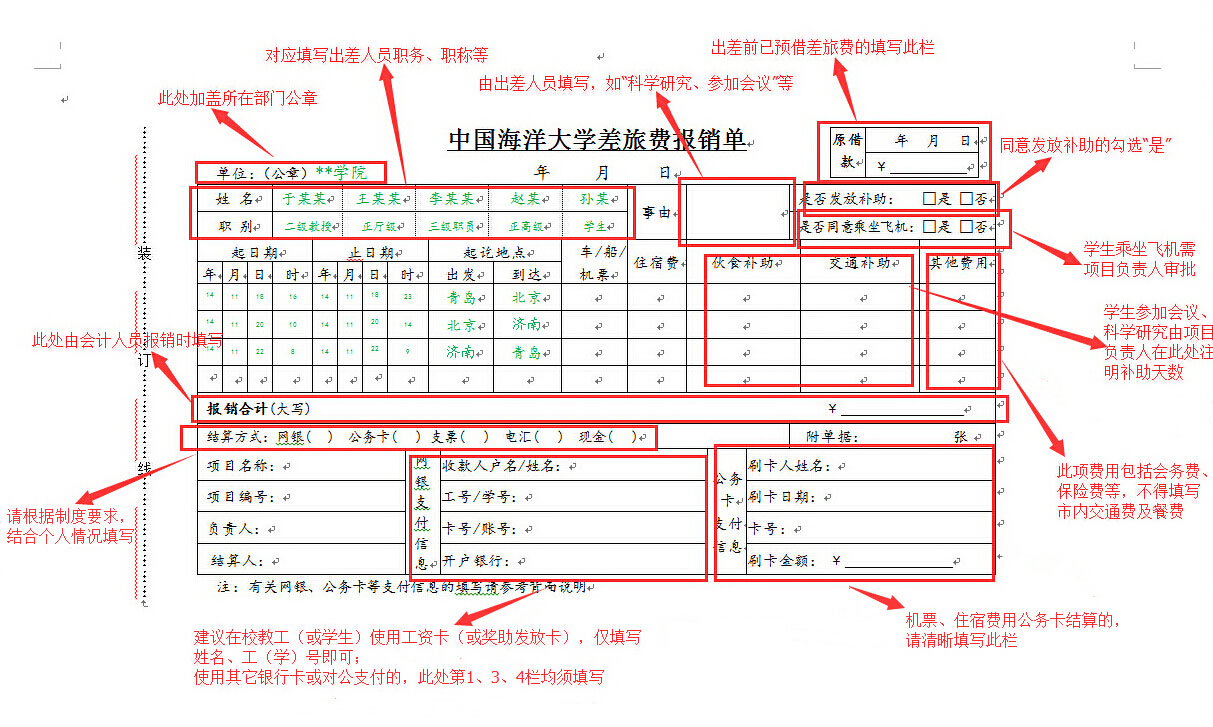
\includegraphics[width=4.0in]{baoxiao} \caption{填写图解}
\end{minipage}	
\begin{minipage}[c]{\textwidth}\centering
	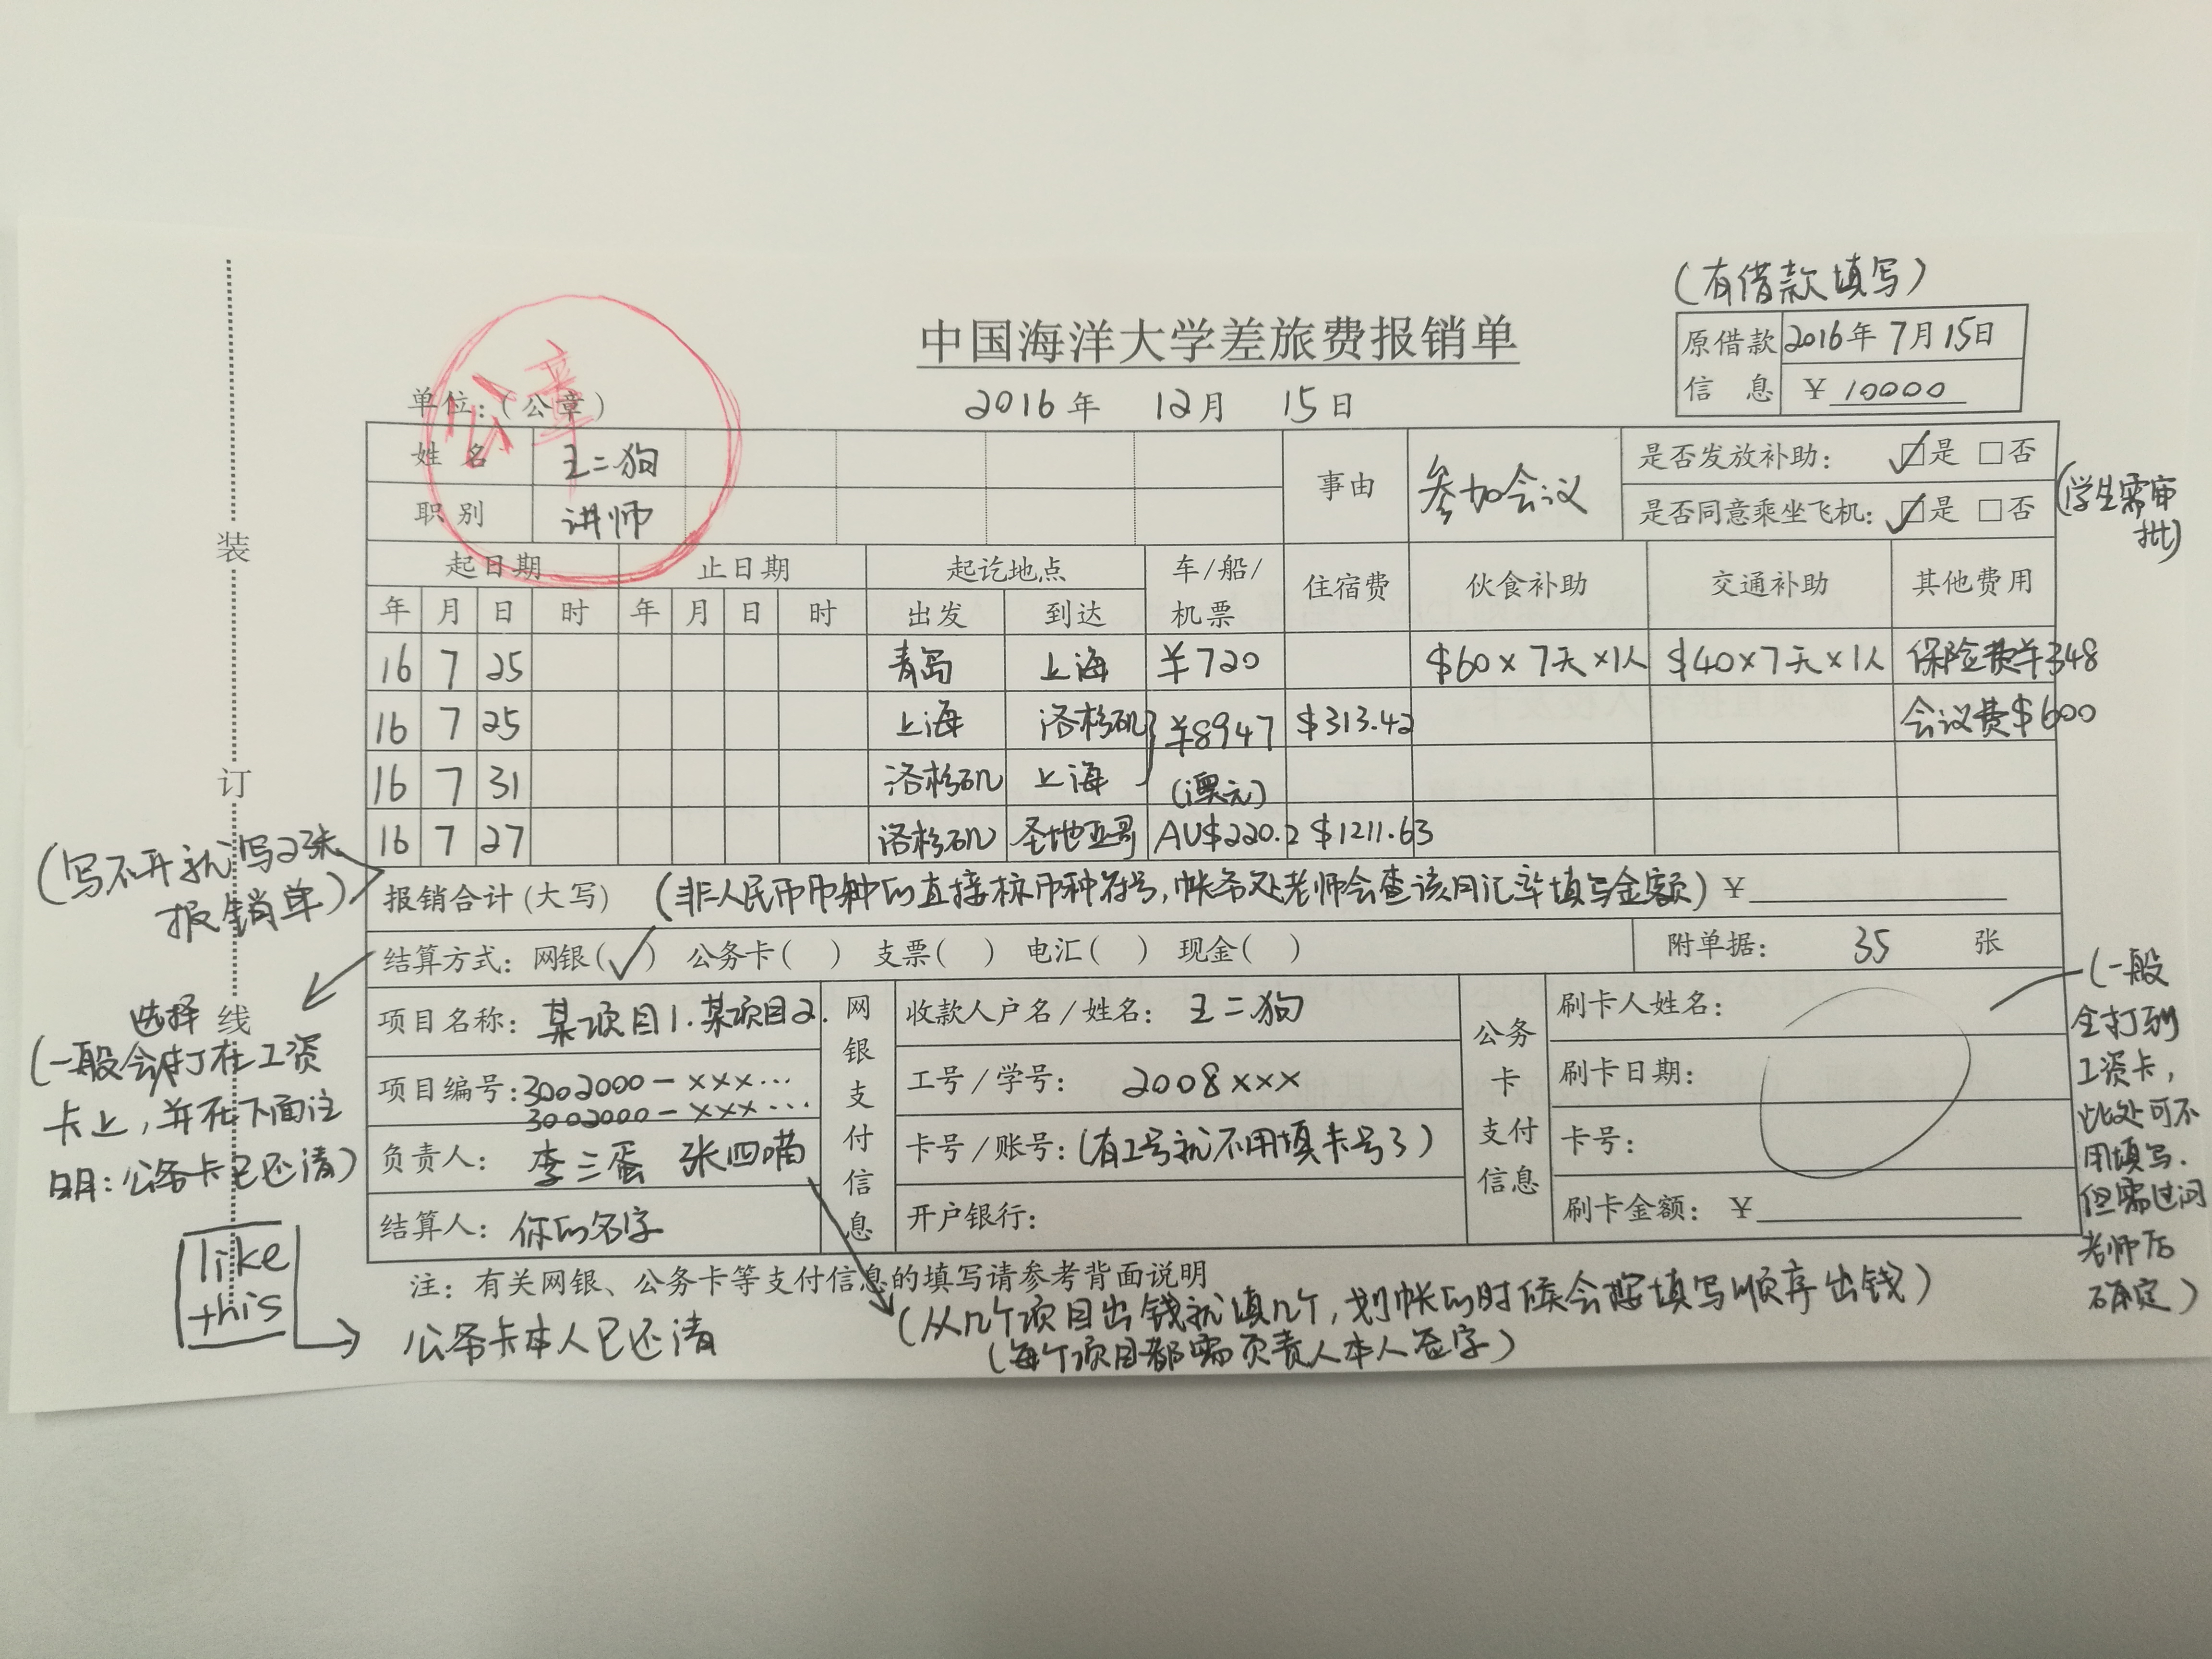
\includegraphics[width=4.0in]{baoxiao2}\caption{报销单参考}
\end{minipage}

\end{figure}\\
	如图,费用可以不全为人民币,但需要表明币种符号,注意多币种都使用了\$符号,除美元外都需中文标注。项目名称可以简写几个字代替,但项目编号必须完整,负责人为项目编号对应的负责人而非报账人,有两个不同老师的项目的,需两位老师分别签字。老师的卡号无需填写,可以只填工号。报销单需要盖院办章(407姜斌主任办公室)。\\


\item 借款单据:需要附借款单,如需借款支票,需在财务处用发票换取。【支票不能折!】
\item 机票行程单、登机牌,机票的支付记录
\item 住宿费发票,住宿的支付记录
\item 会议注册费发票,注册费的支付记录
\item 城市间交通费(注明起始地点),其支付记录
\item 签证费、保险费,其支付记录
\item 出国审批表、出国预算审批表、因公出国批件、出国护照复印件、签证复印件(包括签证页和出入境记录页两部分,必须有签证时间那一页)、用汇核销及国外费用支出明细表【这里也要按顺序整理!】
\begin{itemize}
\item[-] 各费用支付记录需附在每一个项目后面,同一张银行支付记录上有几项的内容的,比如机票和住宿都在同一张记录上,可以统一放在机票和宾馆单据后面,但应尽量的分开。支付记录上要将报销的项目圈出来,中文标注姓名、项目内容,如:郑海永拉斯维加斯住宿,或戴嘉伦青岛到上海飞机。
\item[-] 所有发票背面需要有两个经办人的签字。
\item[-] 整理好的单据,可以把同一类的单据贴在一起,不能遮挡信息,不能使用订书钉。
\item[-] 将所有的单据中重要的姓名、地点、时间等信息圈出来,每份单据右上角标注一下单据内容,如:台北3晚住宿发票,或下面这2张为保险单等等。【原则就是,你的标注越方便审账老师,老师就越方便你,不然万一人家就愿意跟你说一个问题把你赶走,下次去再说第二个,那就只能一直泪奔在行远路上了】
\end{itemize}
\end{itemize}
\item 报销单上项目可能与预审时申报项目不一致,需要写一份说明(手写即可,负责人签字,盖院办章)。原因可填写:项目经费不够、某一个项目即将到期等原因。
\item 未乘坐国内航空公司飞机的行程都需要预先审批,附一份《乘坐非国内航空公司航班和改变中转地审批表》。这个表是由出国人员在出国前准备的,若没有需填写特殊事项申请表\url{http://cwc.ouc.edu.cn/upfiles/news/20160901161116884.doc},表中说明为什么没有提前审批和乘坐外国航班的原因(几段外国航空公司的行程就需填写几张表,负责人签字,盖院办章)。
\item 所有英文材料,需要把票据上重要信息圈出,用中文手写票据内容、日期、数量、金额(币种用中文写完整,勿用货币符号)等,并由经办人在旁边签字。
\item 明细表、报销单等重要表单上面的任何涂改,经办人需要在旁边签字。
\end{enumerate}
\textbf{二、财务处报账流程}:
\begin{enumerate}
\item 拿着你整理好的,用漂亮的小夹子整整齐齐夹好的单据自信的迈进宽敞明亮的报账大厅。
\item 经过审阅,财务处老师发现你的材料准确无误,会带着迷人的微笑帮忙打印一份《临时出国团组(人员)费用人民币结算表》,认真的对照一下老师是否打错了某笔金额,没问题就可以回实验室了。
\item 从财务处官网打印《出国(境)人员用汇核销及费用支出明细表》\url{http://cwc.ouc.edu.cn/upfiles/news/20150403165526731.doc},按照《结算表》认真填写好表格,附在最后一张(主任签字,盖院办章)。
\item 《结算表》左下角的内容需要填写,报账单上写的是工资卡就填写在工资卡一栏,不止一个人的可以另起一行填写,写明给每个人打的钱数具体是多少。【建议:如果老师同意,还是写一个人方便一些,打完钱再让报销者自己分赃。。不不不,是分钱】
\item 拿好所有材料,趁没隔几天的老师对账还有印象的时候去第二次,这次简单看一下没问题,老师就会帮忙打两张小表单,跟你说你可以回家了。
\item 报账圆满完成。
\item[Tips] 以上当然是清醒梦的内容。下面聊点实际的:
\begin{itemize}
\item 报账这件事是需要抢的,因为一份很厚的账老师可能就要一审两个多小时,所以能第一个到财务处就别第二个。【按照经验,平时的话8:30前去就能排第一,年终的时候则一天比一天恐怖,6:30到也排不到第一】
\item 财务处上班时间:8:00-11:30, 13:30-17:00。进门不要犹豫,先到右手边找取号机,点一下外汇按钮取票。虽应尽量避免,但如果不幸拖到了年终报账,可以找人一起早起,然后领好几个不相邻的号码。
\item 最好不要一个人去报外汇!因为一次成功是需要天时地利人和的,如果需要补交材料签字等等,可以让另一个人快速跑腿办理,材料写的不全的,在账多的时候两个人一起填也是可以快一倍的。
\end{itemize}
\end{enumerate}
\end{document}
